% answers.tex —— 2010 年·普通高等学校招生考试·辽宁卷·文科 · 参考答案与详细解析片段
% 由 tools/generate_projects.py 依来源总账自 2010/2010_数学真题_辽宁文_试题.md + 2010/2010_数学真题_辽宁文_解析正文.md + 2010/2010_数学真题_辽宁文_答案要点.md 生成，勿手改（改源 MD 后重跑）

\begin{gktip}
固定候选 PDF 仅含题面、无答案页；以下解析与结论均由本库独立推导（非官方答案），并按 600 dpi 原页复核题面。原页未印分值，不补。

【源疑点】原页第 22–24 题紧接第 21 题排在同一条「三、解答题」之下，未另印「选考题」栏目名，也未标「三选一」；按课标卷体例这三题分属几何证明选讲、坐标系与参数方程、不等式选讲，属选考。此处照录，不改栏目名。
\end{gktip}

\begin{answer}
\gksolhead{1}{}

\textbf{题目}：

已知集合 $U=\{1,3,5,7,9\}$，$A=\{1,5,7\}$，则 $\complement_U A=$（　）

（A）$\{1,3\}$

（B）$\{3,7,9\}$

（C）$\{3,5,9\}$

（D）$\{3,9\}$

\Needspace{4\baselineskip}
\textbf{解析}
\Needspace{5\baselineskip}
$U=\{1,3,5,7,9\}$，$A=\{1,5,7\}$。补集是 $U$ 中不属于 $A$ 的元素全体，即
\nopagebreak[4]
\[\complement_U A=\{3,9\}.\]
逐项核对：A 项 $\{1,3\}$ 含 $1\in A$；B 项 $\{3,7,9\}$ 含 $7\in A$；C 项 $\{3,5,9\}$ 含 $5\in A$；只有 D 项与计算结果一致，且 $3+9=12$、$|A|+|\complement_UA|=3+2=5=|U|$，数目也吻合。
故选 D。

\gkanswer{答案：D。}

\end{answer}
\begin{answer}
\gksolhead{2}{}

\textbf{题目}：

设 $a$，$b$ 为实数，若复数 $\dfrac{1+2\mathrm i}{a+b\mathrm i}=1+\mathrm i$，则（　）

（A）$a=\dfrac32$，$b=\dfrac12$

（B）$a=3$，$b=1$

（C）$a=\dfrac12$，$b=\dfrac32$

（D）$a=1$，$b=3$

\Needspace{4\baselineskip}
\textbf{解析}
\Needspace{5\baselineskip}
两边乘 $a+b\mathrm i$：
\nopagebreak[4]
\[1+2\mathrm i=(1+\mathrm i)(a+b\mathrm i)=(a-b)+(a+b)\mathrm i.\]
\Needspace{5\baselineskip}
比较实部、虚部得
\nopagebreak[4]
\[a-b=1,\qquad a+b=2,\]
解得 $a=\dfrac32$，$b=\dfrac12$。
\Needspace{5\baselineskip}
代回检验：
\nopagebreak[4]
\[\frac{1+2\mathrm i}{\dfrac32+\dfrac12\mathrm i}
=\frac{(1+2\mathrm i)\left(\dfrac32-\dfrac12\mathrm i\right)}
{\left(\dfrac32\right)^2+\left(\dfrac12\right)^2}
=\frac{\dfrac52+\dfrac52\mathrm i}{\dfrac52}=1+\mathrm i,\]
与题意相符。其余三项均不能使商为 $1+\mathrm i$：
\begin{itemize}
\item B 项：$\dfrac{1+2\mathrm i}{3+\mathrm i}=\dfrac{(1+2\mathrm i)(3-\mathrm i)}{10}=\dfrac12+\dfrac12\mathrm i$；
\item C 项：$\dfrac{1+2\mathrm i}{\dfrac12+\dfrac32\mathrm i}=\dfrac{(1+2\mathrm i)\left(\dfrac12-\dfrac32\mathrm i\right)}{\dfrac14+\dfrac94}=\dfrac{\dfrac72-\dfrac12\mathrm i}{\dfrac52}=\dfrac75-\dfrac15\mathrm i$；
\item D 项：$\dfrac{1+2\mathrm i}{1+3\mathrm i}=\dfrac{(1+2\mathrm i)(1-3\mathrm i)}{10}=\dfrac7{10}-\dfrac1{10}\mathrm i$。
\end{itemize}
故选 A。

\gkanswer{答案：A。}

\end{answer}
\begin{answer}
\gksolhead{3}{}

\textbf{题目}：

设 $S_n$ 为等比数列 $\{a_n\}$ 的前 $n$ 项和，已知 $3S_3=a_4-2$，$3S_2=a_3-2$，则公比 $q=$（　）

（A）$3$

（B）$4$

（C）$5$

（D）$6$

\Needspace{4\baselineskip}
\textbf{解析}
\Needspace{5\baselineskip}
由 $S_3=S_2+a_3$，两式相减得
\nopagebreak[4]
\[3S_3-3S_2=(a_4-2)-(a_3-2)\iff3a_3=a_4-a_3,\]
即 $a_4=4a_3$。等比数列中 $a_3\neq0$（各项均非零），故 $q=\dfrac{a_4}{a_3}=4$。
\Needspace{5\baselineskip}
代回验证存在性：设 $a_1=2$，$q=4$，则 $a_3=32$，$a_4=128$，$S_2=10$，$S_3=42$，
\nopagebreak[4]
\[3S_2=30=a_3-2=30,\qquad 3S_3=126=a_4-2=126,\]
两式同时成立，故 $q=4$ 确实可行。
逐项核对：$q=3$ 时由两式相减得 $a_4=4a_3$ 不成立；$q=5$、$q=6$ 同理。
故选 B。

\gkanswer{答案：B。}

\end{answer}
\begin{answer}
\gksolhead{4}{}

\textbf{题目}：

已知 $a>0$，函数 $f(x)=ax^2+bx+c$。若 $x_0$ 满足关于 $x$ 的方程 $2ax+b=0$，则下列选项的命题中为假命题的是（　）

（A）$\exists x\in\mathbf R$，$f(x)\leqslant f(x_0)$

（B）$\exists x\in\mathbf R$，$f(x)\geqslant f(x_0)$

（C）$\forall x\in\mathbf R$，$f(x)\leqslant f(x_0)$

（D）$\forall x\in\mathbf R$，$f(x)\geqslant f(x_0)$

\Needspace{4\baselineskip}
\textbf{解析}
\Needspace{5\baselineskip}
由 $2ax+b=0$ 得 $x_0=-\dfrac{b}{2a}$。因 $a>0$，$f(x)=ax^2+bx+c$ 的图象开口向上，$x_0$ 就是对称轴，也是 $f$ 在 $\mathbf R$ 上的最小值点，故
\nopagebreak[4]
\[\forall x\in\mathbf R,\quad f(x)\geqslant f(x_0),\]
即 D 是真命题。取 $x=x_0$ 可知 $f(x)\leqslant f(x_0)$ 与 $f(x)\geqslant f(x_0)$ 都能成立，故 A、B 也是真命题（存在性命题只需一个实例）。
而 C 断言对一切 $x$ 有 $f(x)\leqslant f(x_0)$，即 $f(x_0)$ 为最大值；但 $f(x)=a\left(x-x_0\right)^2+f(x_0)$，当 $x\neq x_0$ 时 $f(x)>f(x_0)$，故 C 是假命题。
故选 C。

\gkanswer{答案：C。}

\end{answer}
\begin{answer}
\gksolhead{5}{}

\textbf{题目}：

如果执行下图所示的程序框图，输入 $n=6$，$m=4$，那么输出的 $p$ 等于（　）

（A）$720$

（B）$360$

（C）$240$

（D）$120$
\nopagebreak[4]
\begin{center}% 2010 年辽宁卷文科第 5 题：程序框图（累乘，输出 p）。
% 来源 PDF：普通高考/2010/2010辽宁文.pdf，SHA-256 b402a859318cb9854e9b8257ea128e84f1d52e834556dd80625e883f88dea1fd。
% 原页：第 1 页（A3 三栏）第 1 栏中部偏下，书页码 613。
% 重绘依据：照原页竖排主干 开始→输入 n,m→k=1,p=1→p=p(n-m+k)→判断 k<m?
%   「是」向右再向上进入右侧 k=k+1 框，该框顶部再向左汇入 p=p(n-m+k) 上方主干（循环体为
%   p=p(n-m+k)、k=k+1）；「否」向下经「输出 p」到「结束」。原页题干写「下图所示」。
\begin{tikzpicture}[semithick,
  every node/.style={inner sep=2pt},
  box/.style={draw, minimum width=3.7cm, minimum height=0.62cm, align=center},
  round/.style={draw, rounded corners=6pt, minimum width=1.7cm,
    minimum height=0.62cm, align=center},
  para/.style={draw, trapezium, trapezium left angle=70, trapezium right angle=110,
    minimum width=2.5cm, minimum height=0.66cm, align=center},
  dec/.style={draw, diamond, aspect=2.2, minimum width=2.6cm,
    minimum height=1.05cm, align=center},
  arr/.style={->, >=stealth}]

  \node[round] (start) at (0,0) {开始};
  \node[para]  (in)    at (0,-1.15) {输入 $n,\,m$};
  \node[box]   (init)  at (0,-2.32) {$k=1$，$p=1$};
  \node[box]   (prod)  at (0,-3.62) {$p=p(n-m+k)$};
  \node[box]   (inc)   at (4.15,-3.62) {$k=k+1$};
  \node[dec]   (test)  at (0,-5.05) {$k<m$};
  \node[para]  (out)   at (0,-6.40) {输出 $p$};
  \node[round] (end)   at (0,-7.50) {结束};

  \draw[arr] (start) -- (in);
  \draw[arr] (in) -- (init);
  \draw[arr] (init) -- (prod);
  \draw[arr] (test) -- (out);
  \node[right] at (0.18,-5.85) {否};
  \draw[arr] (out) -- (end);

  % 「是」分支：由判断框右侧向右、再向上进入 k=k+1
  \draw[arr] (test.east) -| (inc.south);
  \node[above] at (1.65,-5.03) {是};

  % 回边：k=k+1 顶部向上、再向左汇入 p=p(n-m+k) 上方主干
  \draw (inc.north) -- (4.15,-2.95) -- (0,-2.95);
\end{tikzpicture}
\end{center}
\nopagebreak[4]
\Needspace{4\baselineskip}
\textbf{解析}
按框图追踪变量。$n=6$，$m=4$，初值 $k=1$，$p=1$。

\begin{center}
\begin{tabular}{llll}
\toprule
轮次 & 执行 $p\leftarrow p(n-m+k)$ & 判断 $k<m$ & 下一步 \\
\midrule
1 & $p=1\times(6-4+1)=3$ & $1<4$ 是 & $k=2$ \\
2 & $p=3\times(6-4+2)=12$ & $2<4$ 是 & $k=3$ \\
3 & $p=12\times(6-4+3)=60$ & $3<4$ 是 & $k=4$ \\
4 & $p=60\times(6-4+4)=360$ & $4<4$ 否 & 输出 $p$ \\
\bottomrule
\end{tabular}
\end{center}

故输出 $p=3\times4\times5\times6=360$。
一般地，$p$ 依次乘上 $n-m+1,n-m+2,\cdots,n$ 共 $m$ 个连续整数，即 $\mathrm A_n^m$；本题 $\mathrm A_6^4=6\times5\times4\times3=360$。逐项核对：$720=6!$（多乘了 $1,2$），$120=5!$，$240$ 不是四个连续整数之积。
故选 B。

\gkanswer{答案：B。}

\end{answer}
\begin{answer}
\gksolhead{6}{}

\textbf{题目}：

设 $\omega>0$，函数 $y=\sin\left(\omega x+\dfrac{\pi}{3}\right)+2$ 的图象向右平移 $\dfrac{4\pi}{3}$ 个单位后与原图象重合，则 $\omega$ 的最小值是（　）

（A）$\dfrac23$

（B）$\dfrac43$

（C）$\dfrac32$

（D）$3$

\Needspace{4\baselineskip}
\textbf{解析}
\Needspace{5\baselineskip}
图象向右平移 $\dfrac{4\pi}{3}$ 个单位后为
\nopagebreak[4]
\[y=\sin\left[\omega\left(x-\frac{4\pi}{3}\right)+\frac{\pi}{3}\right]+2
=\sin\left(\omega x+\frac{\pi}{3}-\frac{4\pi\omega}{3}\right)+2.\]
\Needspace{5\baselineskip}
与原图象重合，等价于初相之差是 $2\pi$ 的整数倍：
\nopagebreak[4]
\[\frac{4\pi\omega}{3}=2k\pi\quad(k\in\mathbf Z)\iff\omega=\frac{3k}{2}.\]
由 $\omega>0$ 得 $k\geqslant1$，故 $\omega$ 的最小值为 $\dfrac32$（$k=1$）。此时平移量恰为一个周期 $\dfrac{2\pi}{\omega}=\dfrac{4\pi}{3}$。
逐项核对：$\omega=\dfrac23$ 时平移量为 $2\pi\cdot\dfrac{2}{9}$，非周期整数倍；$\dfrac43$、$3$ 同样不满足 $\omega=\dfrac{3k}{2}$（$k$ 为整数）。
故选 C。

\gkanswer{答案：C。}

\end{answer}
\begin{answer}
\gksolhead{7}{}

\textbf{题目}：

设抛物线 $y^2=8x$ 的焦点为 $F$，准线为 $l$，$P$ 为抛物线上一点，$PA\perp l$，$A$ 为垂足，如果直线 $AF$ 的斜率为 $-\sqrt3$，那么 $|PF|=$（　）

（A）$4\sqrt3$

（B）$8$

（C）$8\sqrt3$

（D）$16$

\Needspace{4\baselineskip}
\textbf{解析}
$y^2=8x$ 中 $2p=8$，$p=4$，焦点 $F(2,0)$，准线 $l:x=-2$。
\Needspace{5\baselineskip}
设 $A(-2,y_0)$（$A$ 在准线上），则
\nopagebreak[4]
\[k_{AF}=\frac{y_0-0}{-2-2}=-\frac{y_0}{4}=-\sqrt3\iff y_0=4\sqrt3.\]
于是 $P$ 的纵坐标为 $4\sqrt3$，代入 $y^2=8x$ 得 $x_P=\dfrac{48}{8}=6$。
\Needspace{5\baselineskip}
由抛物线定义，$|PF|$ 等于 $P$ 到准线的距离，即
\nopagebreak[4]
\[|PF|=|PA|=x_P-(-2)=6+2=8.\]
逐项核对：$4\sqrt3\approx6.93$，$8\sqrt3\approx13.86$，$16$ 均与 $8$ 不符。
故选 B。

\gkanswer{答案：B。}

\end{answer}
\begin{answer}
\gksolhead{8}{}

\textbf{题目}：

平面上 $O$，$A$，$B$ 三点不共线，设 $\overrightarrow{OA}=\boldsymbol a$，$\overrightarrow{OB}=\boldsymbol b$，则 $\triangle OAB$ 的面积等于（　）

（A）$\sqrt{|\boldsymbol a|^2|\boldsymbol b|^2-(\boldsymbol a\cdot\boldsymbol b)^2}$

（B）$\sqrt{|\boldsymbol a|^2|\boldsymbol b|^2+(\boldsymbol a\cdot\boldsymbol b)^2}$

（C）$\dfrac12\sqrt{|\boldsymbol a|^2|\boldsymbol b|^2-(\boldsymbol a\cdot\boldsymbol b)^2}$

（D）$\dfrac12\sqrt{|\boldsymbol a|^2|\boldsymbol b|^2+(\boldsymbol a\cdot\boldsymbol b)^2}$

\Needspace{4\baselineskip}
\textbf{解析}
\Needspace{5\baselineskip}
设 $\boldsymbol a$、$\boldsymbol b$ 的夹角为 $\theta\in(0,\pi)$（三点不共线保证 $\theta\neq0,\pi$）。三角形面积
\nopagebreak[4]
\[S_{\triangle OAB}=\frac12|\boldsymbol a||\boldsymbol b|\sin\theta.\]
\Needspace{5\baselineskip}
而
\nopagebreak[4]
\[|\boldsymbol a|^2|\boldsymbol b|^2-(\boldsymbol a\cdot\boldsymbol b)^2
=|\boldsymbol a|^2|\boldsymbol b|^2-|\boldsymbol a|^2|\boldsymbol b|^2\cos^2\theta
=|\boldsymbol a|^2|\boldsymbol b|^2\sin^2\theta,\]
\Needspace{5\baselineskip}
开方即 $|\boldsymbol a||\boldsymbol b|\sin\theta$（$\sin\theta>0$），故
\nopagebreak[4]
\[S=\frac12\sqrt{|\boldsymbol a|^2|\boldsymbol b|^2-(\boldsymbol a\cdot\boldsymbol b)^2}.\]
逐项核对：A、B 少了因子 $\dfrac12$；D 的根号内是加号，$|\boldsymbol a|^2|\boldsymbol b|^2+(\boldsymbol a\cdot\boldsymbol b)^2$ 无法化为面积的平方。
数值验证：取 $\boldsymbol a=(1,0)$，$\boldsymbol b=(0,1)$，则 $S=\dfrac12$，选项 C 给 $\dfrac12\sqrt{1-0}=\dfrac12$，其余三项分别给 $1,1,\dfrac{\sqrt2}{2}$。
故选 C。

\gkanswer{答案：C。}

\end{answer}
\begin{answer}
\gksolhead{9}{}

\textbf{题目}：

设双曲线的一个焦点为 $F$，虚轴的一个端点为 $B$，如果直线 $FB$ 与该双曲线的一条渐近线垂直，那么此双曲线的离心率为（　）

（A）$\sqrt2$

（B）$\sqrt3$

（C）$\dfrac{\sqrt3+1}{2}$

（D）$\dfrac{\sqrt5+1}{2}$

\Needspace{4\baselineskip}
\textbf{解析}
\Needspace{5\baselineskip}
设双曲线 $\dfrac{x^2}{a^2}-\dfrac{y^2}{b^2}=1$，则 $F(c,0)$，虚轴端点 $B(0,b)$，
\nopagebreak[4]
\[k_{FB}=\frac{b-0}{0-c}=-\frac bc.\]
\Needspace{5\baselineskip}
两条渐近线的斜率为 $\pm\dfrac ba$。与 $k_{FB}$ 垂直的只能是斜率为 $\dfrac ba$ 的那条（另一条斜率为 $-\dfrac ba$，乘积为正，不可能垂直），故
\nopagebreak[4]
\[\left(-\frac bc\right)\cdot\frac ba=-1\iff b^2=ac.\]
\Needspace{5\baselineskip}
由 $c^2=a^2+b^2$ 得 $c^2-a^2=ac$，两边除以 $a^2$ 并记 $e=\dfrac ca$：
\nopagebreak[4]
\[e^2-e-1=0\iff e=\frac{1+\sqrt5}{2}\ (\text{\text{舍负根}}).\]
逐项核对：$e=\sqrt2$ 时 $b^2=a^2$，$ac=\sqrt2a^2$，不满足；$e=\sqrt3$ 时 $b^2=2a^2$，$ac=\sqrt3a^2$，不满足；$e=\dfrac{\sqrt3+1}{2}$ 时 $e^2-e=\dfrac{2+\sqrt3}{2}-\dfrac{\sqrt3+1}{2}=\dfrac12\neq1$，不满足。
故选 D。

\gkanswer{答案：D。}

\end{answer}
\begin{answer}
\gksolhead{10}{}

\textbf{题目}：

设 $2^a=5^b=m$，且 $\dfrac1a+\dfrac1b=2$，则 $m=$（　）

（A）$\sqrt{10}$

（B）$10$

（C）$20$

（D）$100$

\Needspace{4\baselineskip}
\textbf{解析}
\Needspace{5\baselineskip}
由 $2^a=5^b=m$ 知 $m>0$ 且 $m\neq1$，取对数
\nopagebreak[4]
\[a=\frac{\ln m}{\ln2},\qquad b=\frac{\ln m}{\ln5},\]
\Needspace{5\baselineskip}
故
\nopagebreak[4]
\[\frac1a+\frac1b=\frac{\ln2}{\ln m}+\frac{\ln5}{\ln m}=\frac{\ln10}{\ln m}=2,\]
从而 $\ln m=\dfrac12\ln10$，$m=\sqrt{10}$。
代回检验：$2^a=5^b=\sqrt{10}$ 给出 $a=\log_2\sqrt{10}\approx1.66$，$b=\log_5\sqrt{10}\approx0.72$，$\dfrac1a+\dfrac1b\approx0.602+1.398=2$，符合。
逐项核对：$m=10$ 时 $\dfrac1a+\dfrac1b=\dfrac{\ln10}{\ln10}=1$；$m=100$ 时为 $\dfrac12$；$m=20$ 时 $\dfrac{\ln10}{\ln20}\approx0.77$。
故选 A。

\gkanswer{答案：A。}

\end{answer}
\begin{answer}
\gksolhead{11}{}

\textbf{题目}：

已知 $S$，$A$，$B$，$C$ 是球 $O$ 表面上的点，$SA\perp$ 平面 $ABC$，$AB\perp BC$，$SA=AB=1$，$BC=\sqrt2$，则球 $O$ 的表面积等于（　）

（A）$4\pi$

（B）$3\pi$

（C）$2\pi$

（D）$\pi$

\Needspace{4\baselineskip}
\textbf{解析}
$\triangle ABC$ 中 $AB\perp BC$，$AB=1$，$BC=\sqrt2$，故 $AC=\sqrt3$，外接圆圆心为斜边 $AC$ 的中点，半径 $\dfrac{\sqrt3}{2}$。
\Needspace{5\baselineskip}
因 $SA\perp$ 平面 $ABC$，可设 $A$ 为原点，$AB$、$BC$、$AS$ 方向为坐标轴（$AB\perp BC$、$AS\perp$ 平面 $ABC$ 保证三轴两两垂直）：
\nopagebreak[4]
\[A(0,0,0),\quad B(1,0,0),\quad C(1,\sqrt2,0),\quad S(0,0,1).\]
\Needspace{5\baselineskip}
设球心 $O(x,y,z)$。由 $OA=OB=OC$ 得 $O$ 在 $\triangle ABC$ 的外心正上方，即 $(x,y)=\left(\dfrac12,\dfrac{\sqrt2}{2}\right)$；由 $OA=OS$ 得
\nopagebreak[4]
\[\frac14+\frac12+z^2=\frac14+\frac12+(z-1)^2\iff z=\frac12.\]
\Needspace{5\baselineskip}
于是
\nopagebreak[4]
\[R^2=OA^2=\frac14+\frac12+\frac14=1,\]
球 $O$ 的表面积为 $4\pi R^2=4\pi$。
逐项核对：$3\pi$、$2\pi$、$\pi$ 对应的半径分别为 $\dfrac{\sqrt3}{2}$、$\dfrac{\sqrt2}{2}$、$\dfrac12$，均与 $R=1$ 不符。
故选 A。

\gkanswer{答案：A。}

\end{answer}
\begin{answer}
\gksolhead{12}{}

\textbf{题目}：

已知点 $P$ 在曲线 $y=\dfrac{4}{\mathrm e^x+1}$ 上，$\alpha$ 为曲线在点 $P$ 处的切线的倾斜角，则 $\alpha$ 的取值范围是（　）

（A）$\left[0,\dfrac{\pi}{4}\right)$

（B）$\left[\dfrac{\pi}{4},\dfrac{\pi}{2}\right)$

（C）$\left(\dfrac{\pi}{2},\dfrac{3\pi}{4}\right]$

（D）$\left[\dfrac{3\pi}{4},\pi\right)$

\Needspace{4\baselineskip}
\textbf{解析}
\nopagebreak[4]
\[y=\frac{4}{\mathrm e^x+1},\qquad y'=-\frac{4\mathrm e^x}{(\mathrm e^x+1)^2}.\]
\Needspace{5\baselineskip}
令 $u=\mathrm e^x>0$，则切线斜率
\nopagebreak[4]
\[k=y'=-\frac{4u}{(u+1)^2}=-\frac{4}{u+\dfrac1u+2}.\]
\Needspace{5\baselineskip}
由 $u+\dfrac1u\geqslant2$（$u=1$ 时取等）得 $u+\dfrac1u+2\geqslant4$，且 $u+\dfrac1u+2$ 可取遍 $[4,+\infty)$，故
\nopagebreak[4]
\[k\in[-1,0).\]
\Needspace{5\baselineskip}
又 $\alpha\in[0,\pi)$ 且 $\tan\alpha=k$，在 $\left[\dfrac{3\pi}{4},\pi\right)$ 上 $\tan$ 单调递增且值域为 $[-1,0)$，故
\nopagebreak[4]
\[\alpha\in\left[\frac{3\pi}{4},\pi\right).\]
逐项核对：$\left[0,\dfrac\pi4\right)$ 对应 $k\in[0,1)$，符号错；$\left[\dfrac\pi4,\dfrac\pi2\right)$ 对应 $k\in[1,+\infty)$；$\left(\dfrac\pi2,\dfrac{3\pi}{4}\right]$ 对应 $k\in\left(-\infty,-1\right]$，边界 $-1$ 应取到。
故选 D。

\gkanswer{答案：D。}

\end{answer}
\begin{answer}
\gksolhead{13}{}

\textbf{题目}：

三张卡片上分别写上字母 $E$，$E$，$B$，将三张卡片随机地排成一行，恰好排成英文单词 $BEE$ 的概率为 $\underline{\qquad}$。

\Needspace{4\baselineskip}
\textbf{解析}
\Needspace{5\baselineskip}
把两张写 $E$ 的卡片记为 $E_1$、$E_2$，与 $B$ 一起随机排成一行，共有 $3!=6$ 个基本事件，每个概率为 $\dfrac16$：
\nopagebreak[4]
\[BE_1E_2,\ BE_2E_1,\ E_1BE_2,\ E_2BE_1,\ E_1E_2B,\ E_2E_1B.\]
\Needspace{5\baselineskip}
其中拼成单词 $BEE$ 的只有 $BE_1E_2$ 与 $BE_2E_1$ 两个，二者互斥，故
\nopagebreak[4]
\[P=\frac16+\frac16=\frac13.\]
（若把两张 $E$ 视为相同，则三种“字面排列”$BEE$、$EBE$、$EEB$ 仍是等可能的，各占 $\dfrac13$，结论一致。）

\gkanswer{答案：$\dfrac13$。}

\end{answer}
\begin{answer}
\gksolhead{14}{}

\textbf{题目}：

设 $S_n$ 为等差数列 $\{a_n\}$ 的前 $n$ 项和，若 $S_3=3$，$S_6=24$，则 $a_9=\underline{\qquad}$。

\Needspace{4\baselineskip}
\textbf{解析}
\Needspace{5\baselineskip}
设首项 $a_1$、公差 $d$。由求和公式
\nopagebreak[4]
\[S_3=3a_1+\frac{3\times2}{2}d=3a_1+3d=3\iff a_1+d=1,\]
\nopagebreak[4]
\[S_6=6a_1+\frac{6\times5}{2}d=6a_1+15d=24.\]
\Needspace{5\baselineskip}
把 $a_1=1-d$ 代入第二式：$6(1-d)+15d=24$，即 $9d=18$，$d=2$，$a_1=-1$。故
\nopagebreak[4]
\[a_9=a_1+8d=-1+16=15.\]
代回检验：$S_3=-1+1+3=3$；$S_6=-1+1+3+5+7+9=24$，与题设完全相符。

\gkanswer{答案：$15$。}

\end{answer}
\begin{answer}
\gksolhead{15}{}

\textbf{题目}：

已知 $-1<x+y<4$ 且 $2<x-y<3$，则 $z=2x-3y$ 的取值范围是 $\underline{\qquad}$。（答案用区间表示）

\Needspace{4\baselineskip}
\textbf{解析}
\Needspace{5\baselineskip}
令 $u=x+y$，$v=x-y$，则 $x=\dfrac{u+v}{2}$，$y=\dfrac{u-v}{2}$，于是
\nopagebreak[4]
\[z=2x-3y=2\cdot\frac{u+v}{2}-3\cdot\frac{u-v}{2}=\frac{5v-u}{2}.\]
\Needspace{5\baselineskip}
由 $-1<u<4$、$2<v<3$ 知
\nopagebreak[4]
\[z>\frac{5\times2-4}{2}=3,\qquad z<\frac{5\times3-(-1)}{2}=8.\]
\Needspace{5\baselineskip}
两端都能无限接近但取不到：令 $v\to2^+$、$u\to4^-$ 得 $z\to3^+$；令 $v\to3^-$、$u\to-1^+$ 得 $z\to8^-$。故
\nopagebreak[4]
\[z\in(3,8).\]
（用线性规划理解：可行域是 $(u,v)$ 平面上的开矩形，线性函数 $z=\dfrac{5v-u}{2}$ 在四个顶点处取到 $\dfrac{5\times2-4}{2}=3$、$\dfrac{5\times2-(-1)}{2}=\dfrac{11}{2}$、$\dfrac{5\times3-4}{2}=\dfrac{11}{2}$、$\dfrac{5\times3-(-1)}{2}=8$，端点 3、8 不可取。）

\gkanswer{答案：$(3,8)$。}

\end{answer}
\begin{answer}
\gksolhead{16}{}

\textbf{题目}：

如图，网格纸的小正方形的边长是 $1$，在其上用粗线画出了某多面体的三视图，则这个多面体最长的一条棱的长为 $\underline{\qquad}$。
\nopagebreak[4]
\begin{center}% 2010 年辽宁卷文科第 16 题：网格纸上的三视图（正视图、侧视图、俯视图）。
% 来源 PDF：普通高考/2010/2010辽宁文.pdf，SHA-256 b402a859318cb9854e9b8257ea128e84f1d52e834556dd80625e883f88dea1fd。
% 原页：第 1 页（A3 三栏）第 2 栏下部，书页码 613。
% 重绘依据：照原页 L 形网格（8 列 × 8 行，左下块占 x=0..4、y=0..4，上部满宽 8 列 × 4 行）：
%   左上是正视图（直角边 2、2，直角在右下，斜边自左下至右上），
%   右上是侧视图（直角边 2、2，直角在左下，斜边自左上至右下），
%   左下是俯视图（边长 2 的正方形加一条自左下至右上的对角线）。
%   网格用细灰线，三视图轮廓用粗黑线。
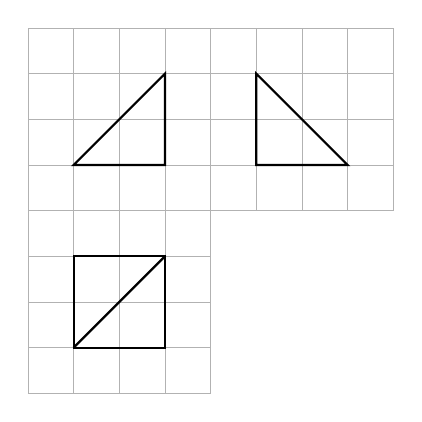
\begin{tikzpicture}[scale=0.58]
  % 横线：上半满宽（x=0..8），下半仅左四列（x=0..4）
  \foreach \y in {0,1,2,3} {
    \draw[gray!60, very thin] (0,\y) -- (4,\y);
  }
  \foreach \y in {4,5,6,7,8} {
    \draw[gray!60, very thin] (0,\y) -- (8,\y);
  }
  % 竖线：左四列满高，右上四列只在上半
  \foreach \x in {0,1,2,3,4} {
    \draw[gray!60, very thin] (\x,0) -- (\x,8);
  }
  \foreach \x in {5,6,7,8} {
    \draw[gray!60, very thin] (\x,4) -- (\x,8);
  }

  % 正视图（左上）：直角边 2、2，斜边自左下至右上
  \draw[thick] (1,5) -- (3,5) -- (3,7) -- cycle;
  % 侧视图（右上）：直角边 2、2，斜边自左上至右下
  \draw[thick] (5,5) -- (7,5) -- (5,7) -- cycle;
  % 俯视图（左下）：边长 2 的正方形加一条对角线
  \draw[thick] (1,1) rectangle (3,3);
  \draw[thick] (1,1) -- (3,3);
\end{tikzpicture}
\end{center}
\nopagebreak[4]
\Needspace{4\baselineskip}
\textbf{解析}
三视图都是“粗线轮廓”，读出各边的格数：正视图是两条直角边都为 $2$ 的直角三角形（直角在右下）；侧视图同样是直角边为 $2$ 的直角三角形（直角在左下）；俯视图是边长 $2$ 的正方形加一条对角线。
由此还原几何体：底面是边长 $2$ 的正方形，顶点在底面某一个顶点的正上方，高为 $2$。验证：设底面 $ABCD$ 中 $A(0,0,0)$、$B(2,0,0)$、$C(2,2,0)$、$D(0,2,0)$，顶点 $P(2,2,2)$，则
\begin{itemize}
\item 正视图（沿 $y$ 方向投影到 $xz$ 面）为 $(0,0),(2,0),(2,2)$ 构成的直角三角形，斜边是棱 $PA$ 的投影；
\item 侧视图（沿 $x$ 方向投影到 $yz$ 面）为 $(0,0),(2,0),(2,2)$ 构成的直角三角形（左视时左右翻转，直角落在左下），斜边同是 $PA$ 的投影；
\item 俯视图为正方形 $ABCD$ 加上棱 $PA$ 的投影，即那条对角线。
\end{itemize}
各棱长：$PA=\sqrt{2^2+2^2+2^2}=2\sqrt3$，$PB=\sqrt{0^2+2^2+2^2}=2\sqrt2$，$PD=\sqrt{2^2+0^2+2^2}=2\sqrt2$，$PC=2$，底面各边为 $2$。故最长棱为 $PA$，长 $2\sqrt3$。

【图注】俯视图只有一条对角线，正说明顶点在其中一个底顶点的正上方（若为四面体，俯视图会出现两条对角线）。顶点选在哪个底顶点只影响图形方向，最长棱恒为 $2\sqrt3$。

\gkanswer{答案：$2\sqrt3$。}

\end{answer}
\begin{answer}
\gksolhead{17}{}

\textbf{题目}：

在 $\triangle ABC$ 中，$a$，$b$，$c$ 分别为内角 $A$，$B$，$C$ 的对边，且 $2a\sin A=(2b+c)\sin B+(2c+b)\sin C$。

（1）求 $A$ 的大小；

（2）若 $\sin B+\sin C=1$，试判断 $\triangle ABC$ 的形状。

\Needspace{4\baselineskip}
\textbf{解析}
\Needspace{5\baselineskip}
（1）由正弦定理 $\dfrac{a}{\sin A}=\dfrac{b}{\sin B}=\dfrac{c}{\sin C}=2R$ 得 $\sin A=\dfrac{a}{2R}$ 等。题设
\nopagebreak[4]
\[2a\sin A=(2b+c)\sin B+(2c+b)\sin C\]
\Needspace{5\baselineskip}
两边乘 $2R$：
\nopagebreak[4]
\[2a^2=(2b+c)b+(2c+b)c=2b^2+2bc+2c^2,\]
\Needspace{5\baselineskip}
即
\nopagebreak[4]
\[a^2=b^2+c^2+bc.\]
\Needspace{5\baselineskip}
与余弦定理 $a^2=b^2+c^2-2bc\cos A$ 比较得
\nopagebreak[4]
\[-2bc\cos A=bc\iff\cos A=-\frac12.\]
\Needspace{5\baselineskip}
因 $A\in(0,\pi)$，故
\nopagebreak[4]
\[A=\frac{2\pi}{3}.\]

\Needspace{5\baselineskip}
（2）由（1）得 $B+C=\dfrac{\pi}{3}$，且 $B,C\in\left(0,\dfrac\pi3\right)$。和差化积：
\nopagebreak[4]
\[\sin B+\sin C=2\sin\frac{B+C}{2}\cos\frac{B-C}{2}
=2\sin\frac{\pi}{6}\cos\frac{B-C}{2}=\cos\frac{B-C}{2}.\]
题设 $\sin B+\sin C=1$，故 $\cos\dfrac{B-C}{2}=1$。因 $\left|\dfrac{B-C}{2}\right|<\dfrac{\pi}{6}$，只有 $B=C$。于是 $B=C=\dfrac{\pi}{6}$，从而 $b=c$，$\triangle ABC$ 是以 $A$ 为顶角（$120^\circ$）的等腰三角形。

\gkanswer{答案：（1）$A=\dfrac{2\pi}{3}$；（2）$\triangle ABC$ 为等腰三角形。}

\end{answer}
\begin{answer}
\gksolhead{18}{}

\textbf{题目}：

为了比较注射 $A$，$B$ 两种药物后产生的皮肤疱疹的面积，选 $200$ 只家兔做试验，将这 $200$ 只家兔随机地分成两组，每组 $100$ 只，其中一组注射药物 $A$，另一组注射药物 $B$。下表 1 和表 2 分别是注射药物 $A$ 和 $B$ 后的试验结果。（疱疹面积单位：$\mathrm{mm}^2$）

表 1：注射药物 $A$ 后皮肤疱疹面积的频数分布表

\begin{center}
\begin{tabular}{llrrr}
\toprule
疱疹面积 & $[60,65)$ & $[65,70)$ & $[70,75)$ & $[75,80)$ \\
\midrule
频数 & $30$ & $40$ & $20$ & $10$ \\
\bottomrule
\end{tabular}
\end{center}

表 2：注射药物 $B$ 后皮肤疱疹面积的频数分布表

\begin{center}
\begin{tabular}{llrrrr}
\toprule
疱疹面积 & $[60,65)$ & $[65,70)$ & $[70,75)$ & $[75,80)$ & $[80,85)$ \\
\midrule
频数 & $10$ & $25$ & $20$ & $30$ & $15$ \\
\bottomrule
\end{tabular}
\end{center}

（1）完成下面频率分布直方图，并比较注射两种药物后疱疹面积的中位数大小；
\nopagebreak[4]
\begin{center}% 2010 年辽宁卷文科第 18 题（1）：两张待完成的频率分布直方图坐标系。
% 来源 PDF：普通高考/2010/2010辽宁文.pdf，SHA-256 b402a859318cb9854e9b8257ea128e84f1d52e834556dd80625e883f88dea1fd。
% 原页：第 1 页（A3 三栏）第 3 栏中部，书页码 613。
% 重绘依据：照原页画空坐标系（原页即要求学生补画小矩形）——纵轴「频率/组距」自
%   0.01 到 0.08，横轴自 0 断裂后为 60 到 85（每 5 一格），纵横虚线网格、两轴各有一处
%   断裂记号；左为图 1：注射药物 A，右为图 2：注射药物 B。不代画柱形，保持与原页一致。
\begin{tikzpicture}[x=0.7cm, y=0.49cm, semithick]
  % ---------- 图 1：注射药物 A ----------
  \begin{scope}
    % 坐标轴
    \draw[->, >=stealth] (0,0) -- (0,9.15);
    \draw[->, >=stealth] (0,0) -- (7.05,0);
    % 虚线网格：竖线 x=1..6（即 60..85），横线 y=1..8（即 0.01..0.08）
    \foreach \i in {1,2,3,4,5,6} {
      \draw[dashed, dash pattern=on 3pt off 3pt] (\i,0) -- (\i,8);
    }
    \foreach \j in {1,2,3,4,5,6,7,8} {
      \draw[dashed, dash pattern=on 3pt off 3pt] (0,\j) -- (6,\j);
    }
    % 纵轴刻度值
    \foreach \j/\v in {1/0.01, 2/0.02, 3/0.03, 4/0.04, 5/0.05, 6/0.06, 7/0.07, 8/0.08} {
      \node[anchor=east, inner sep=1pt] at (-0.12,\j) {\v};
    }
    % 横轴刻度值
    \node[anchor=north, inner sep=2pt] at (0,-0.12) {0};
    \foreach \i/\v in {1/60, 2/65, 3/70, 4/75, 5/80, 6/85} {
      \node[anchor=north, inner sep=2pt] at (\i,-0.12) {\v};
    }
    % 轴断裂记号
    \draw (0.42,0.10) -- (0.56,-0.10) -- (0.70,0.10);
    \draw (0.62,0.10) -- (0.76,-0.10) -- (0.90,0.10);
    \draw (0.10,0.42) -- (-0.10,0.56) -- (0.10,0.70);
    % 轴名
    \node[align=center, inner sep=1pt] at (0.92,10.75) {频率};
    \draw[semithick] (0.36,10.25) -- (1.48,10.25);
    \node[align=center, inner sep=1pt] at (0.92,9.75) {组距};
    \node[anchor=west, inner sep=2pt] at (7.15,1.0) {疱疹面积};
    % 图题
    \node[anchor=north, inner sep=3pt] at (3,-1.05) {图 1：注射药物 $A$};
  \end{scope}

  % ---------- 图 2：注射药物 B ----------
  \begin{scope}[xshift=7.95cm]
    \draw[->, >=stealth] (0,0) -- (0,9.15);
    \draw[->, >=stealth] (0,0) -- (7.05,0);
    \foreach \i in {1,2,3,4,5,6} {
      \draw[dashed, dash pattern=on 3pt off 3pt] (\i,0) -- (\i,8);
    }
    \foreach \j in {1,2,3,4,5,6,7,8} {
      \draw[dashed, dash pattern=on 3pt off 3pt] (0,\j) -- (6,\j);
    }
    \foreach \j/\v in {1/0.01, 2/0.02, 3/0.03, 4/0.04, 5/0.05, 6/0.06, 7/0.07, 8/0.08} {
      \node[anchor=east, inner sep=1pt] at (-0.12,\j) {\v};
    }
    \node[anchor=north, inner sep=2pt] at (0,-0.12) {0};
    \foreach \i/\v in {1/60, 2/65, 3/70, 4/75, 5/80, 6/85} {
      \node[anchor=north, inner sep=2pt] at (\i,-0.12) {\v};
    }
    \draw (0.42,0.10) -- (0.56,-0.10) -- (0.70,0.10);
    \draw (0.62,0.10) -- (0.76,-0.10) -- (0.90,0.10);
    \draw (0.10,0.42) -- (-0.10,0.56) -- (0.10,0.70);
    \node[align=center, inner sep=1pt] at (0.92,10.75) {频率};
    \draw[semithick] (0.36,10.25) -- (1.48,10.25);
    \node[align=center, inner sep=1pt] at (0.92,9.75) {组距};
    \node[anchor=west, inner sep=2pt] at (7.15,1.0) {疱疹面积};
    \node[anchor=north, inner sep=3pt] at (3,-1.05) {图 2：注射药物 $B$};
  \end{scope}
\end{tikzpicture}
\end{center}
\nopagebreak[4]
（2）完成下面 $2\times2$ 列联表，并回答能否有 $99.9\%$ 的把握认为“注射药物 $A$ 后的疱疹面积与注射药物 $B$ 后的疱疹面积有差异”。

\begin{center}
\begin{tabular}{lllr}
\toprule
 & 疱疹面积小于 $70\ \mathrm{mm}^2$ & 疱疹面积不小于 $70\ \mathrm{mm}^2$ & 合计 \\
\midrule
注射药物 $A$ & $a=$ & $b=$ &  \\
注射药物 $B$ & $c=$ & $d=$ &  \\
合计 &  &  & $n=$ \\
\bottomrule
\end{tabular}
\end{center}

\Needspace{5\baselineskip}
附：
\nopagebreak[4]
\[K^2=\frac{n(ad-bc)^2}{(a+b)(c+d)(a+c)(b+d)}.\]

\begin{center}
\begin{tabular}{lrrrrr}
\toprule
$P(K^2\geqslant k)$ & $0.100$ & $0.050$ & $0.025$ & $0.010$ & $0.001$ \\
\midrule
$k$ & $2.706$ & $3.841$ & $5.024$ & $6.635$ & $10.828$ \\
\bottomrule
\end{tabular}
\end{center}

\Needspace{4\baselineskip}
\textbf{解析}
（1）组距为 $5$，各组频率为 $\dfrac{\text{\text{频数}}}{100}$，频率/组距 $=\dfrac{\text{\text{频数}}}{100\times5}=\dfrac{\text{\text{频数}}}{500}$。

\begin{center}
\begin{tabular}{lrrrrr}
\toprule
组别 & $[60,65)$ & $[65,70)$ & $[70,75)$ & $[75,80)$ & $[80,85)$ \\
\midrule
$A$ 频数 & $30$ & $40$ & $20$ & $10$ & — \\
$A$ 频率/组距 & $0.06$ & $0.08$ & $0.04$ & $0.02$ & — \\
$B$ 频数 & $10$ & $25$ & $20$ & $30$ & $15$ \\
$B$ 频率/组距 & $0.02$ & $0.05$ & $0.04$ & $0.06$ & $0.03$ \\
\bottomrule
\end{tabular}
\end{center}

两组频率/组距之和分别为 $0.06+0.08+0.04+0.02=0.20$、$0.02+0.05+0.04+0.06+0.03=0.20$，乘以组距 $5$ 各得 $1$，说明计算无误。

中位数（面积的一半即 $50$ 所在位置）：
\begin{itemize}
\item $A$：前两组累计 $30+40=70\geqslant50$，中位数在 $[65,70)$ 内，$65+\dfrac{50-30}{40}\times5=65+2.5=67.5$；
\item $B$：前三组累计 $10+25+20=55\geqslant50$，中位数在 $[70,75)$ 内，$70+\dfrac{50-35}{20}\times5=70+3.75=73.75$。
\end{itemize}
故 $67.5<73.75$，即注射药物 $A$ 后的疱疹面积的中位数较小。

（2）以 $70$ 为界统计：

\begin{center}
\begin{tabular}{lrrr}
\toprule
 & 小于 $70$ & 不小于 $70$ & 合计 \\
\midrule
注射药物 $A$ & $30+40=70$ & $20+10=30$ & $100$ \\
注射药物 $B$ & $10+25=35$ & $20+30+15=65$ & $100$ \\
合计 & $105$ & $95$ & $200$ \\
\bottomrule
\end{tabular}
\end{center}

\Needspace{5\baselineskip}
即 $a=70$，$b=30$，$c=35$，$d=65$，$n=200$。代入
\nopagebreak[4]
\[K^2=\frac{n(ad-bc)^2}{(a+b)(c+d)(a+c)(b+d)}
=\frac{200(70\times65-30\times35)^2}{100\times100\times105\times95}.\]
\Needspace{5\baselineskip}
其中 $70\times65-30\times35=4550-1050=3500$，故
\nopagebreak[4]
\[K^2=\frac{200\times3500^2}{99750000}=\frac{2450000000}{99750000}\approx24.56.\]
因 $24.56>10.828$，故有 $99.9\%$ 的把握认为“注射药物 $A$ 后的疱疹面积与注射药物 $B$ 后的疱疹面积有差异”。

\gkanswer{答案：（1）频率/组距依次为 $A$：$0.06,0.08,0.04,0.02$，$B$：$0.02,0.05,0.04,0.06,0.03$；中位数 $A$ 为 $67.5$、$B$ 为 $73.75$，故 $A$ 的中位数较小；（2）$a=70$，$b=30$，$c=35$，$d=65$，$n=200$，有 $99.9\%$ 的把握认为有差异。}

\end{answer}
\begin{answer}
\gksolhead{19}{}

\textbf{题目}：

如图，棱柱 $ABC-A_1B_1C_1$ 的侧面 $BCC_1B_1$ 是菱形，$B_1C\perp A_1B$。

（1）证明：平面 $AB_1C\perp$ 平面 $A_1BC_1$；

（2）设 $D$ 是 $A_1C_1$ 上的点，且 $A_1B\parallel$ 平面 $B_1CD$，求 $A_1D:DC_1$ 的值。
\nopagebreak[4]
\begin{center}% 2010 年辽宁卷文科第 19 题：棱柱 ABC-A1B1C1，点 D 在 A1C1 上。
% 来源 PDF：普通高考/2010/2010辽宁文.pdf，SHA-256 b402a859318cb9854e9b8257ea128e84f1d52e834556dd80625e883f88dea1fd。
% 原页：第 2 页（A3 三栏）第 1 栏上部，书页码 614。
% 重绘依据：照原页投影像——A1、C1 在最高处同一水平线上，D 在 A1C1 上（图中居于中点），
%   B1 落在直观图内部；A 在左下、C 在右且与 A 近乎等高，B 在最下方。
%   实线：棱柱可见棱 A1C1、A1A、C1C、A1B1、B1C1、B1B、AB、BC，以及两个辅助平面与截面
%   的边 A1B、BC1、AB1、B1C、B1D；虚线：被遮挡的 AC 与截面边 DC。
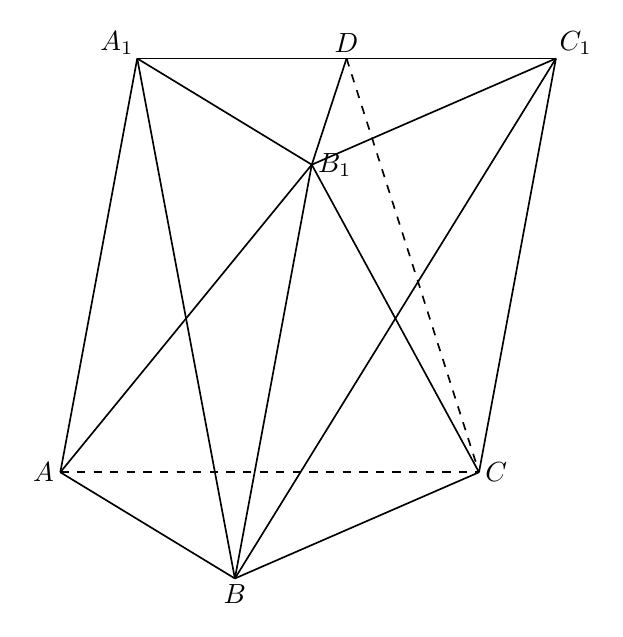
\begin{tikzpicture}[scale=1.55, semithick, line join=round]
  \coordinate (A)  at (0,0);
  \coordinate (B)  at (1.43,-0.87);
  \coordinate (C)  at (3.43,0);
  \coordinate (A1) at (0.63,3.39);
  \coordinate (B1) at (2.06,2.52);
  \coordinate (C1) at (4.06,3.39);
  \coordinate (D)  at (2.345,3.39);

  % 可见棱
  \draw (A1) -- (C1);
  \draw (A1) -- (A);
  \draw (C1) -- (C);
  \draw (A1) -- (B1);
  \draw (B1) -- (C1);
  \draw (B1) -- (B);
  \draw (A) -- (B);
  \draw (B) -- (C);

  % 平面 A1BC1 与平面 AB1C 的边（实线）
  \draw (A1) -- (B);
  \draw (C1) -- (B);
  \draw (A) -- (B1);
  \draw (B1) -- (C);

  % 截面 B1CD（B1D、B1C 已画；DC 被遮挡）
  \draw (B1) -- (D);

  % 被遮挡的棱与线段（虚线）
  \draw[dashed] (A) -- (C);
  \draw[dashed] (D) -- (C);

  % 顶点标注
  \node[above left, inner sep=1pt] at (A1) {$A_1$};
  \node[above, inner sep=2pt] at (D) {$D$};
  \node[above right, inner sep=1pt] at (C1) {$C_1$};
  \node[right=1pt, inner sep=1pt] at (B1) {$B_1$};
  \node[left, inner sep=2pt] at (A) {$A$};
  \node[below, inner sep=2pt] at (B) {$B$};
  \node[right, inner sep=2pt] at (C) {$C$};
\end{tikzpicture}
\end{center}
\nopagebreak[4]
\Needspace{4\baselineskip}
\textbf{解析}
\Needspace{5\baselineskip}
（1）因侧面 $BCC_1B_1$ 是菱形，菱形的对角线互相垂直，故
\nopagebreak[4]
\[B_1C\perp BC_1.\]
\Needspace{5\baselineskip}
又题设 $B_1C\perp A_1B$，而 $BC_1$ 与 $A_1B$ 是平面 $A_1BC_1$ 内两条相交直线（相交于 $B$），所以
\nopagebreak[4]
\[B_1C\perp\text{\text{平面} }A_1BC_1.\]
\Needspace{5\baselineskip}
因 $B_1C\subset$ 平面 $AB_1C$，由面面垂直的判定定理得
\nopagebreak[4]
\[\text{\text{平面} }AB_1C\perp\text{\text{平面} }A_1BC_1.\]

（2）因 $A_1B\parallel$ 平面 $B_1CD$，且 $A_1B\subset$ 平面 $A_1BC_1$，故平面 $A_1BC_1$ 与平面 $B_1CD$ 的交线 $l$ 满足 $l\parallel A_1B$。
又 $D\in A_1C_1\subset$ 平面 $A_1BC_1$ 且 $D\in$ 平面 $B_1CD$，故 $D\in l$，即 $l$ 是平面 $A_1BC_1$ 内过 $D$ 且平行于 $A_1B$ 的直线。设 $l$ 交 $BC_1$ 于 $F$，则 $F\in$ 平面 $B_1CD$。
\Needspace{5\baselineskip}
另一方面，平面 $B_1CD$ 与平面 $BCC_1B_1$ 都经过 $B_1$、$C$，故其交线为 $B_1C$；而 $F\in BC_1\subset$ 平面 $BCC_1B_1$，所以 $F\in B_1C$，即
\nopagebreak[4]
\[F=BC_1\cap B_1C.\]
$F$ 是菱形 $BCC_1B_1$ 两条对角线的交点，也就是 $BC_1$ 的中点。
\Needspace{5\baselineskip}
在 $\triangle C_1A_1B$ 中，$D\in C_1A_1$，$F\in C_1B$，$DF\parallel A_1B$，由相似比
\nopagebreak[4]
\[\frac{C_1D}{C_1A_1}=\frac{C_1F}{C_1B}=\frac12,\]
\Needspace{5\baselineskip}
故 $D$ 是 $A_1C_1$ 的中点，
\nopagebreak[4]
\[A_1D:DC_1=1.\]

【图注】原页图形把 $D$ 画在 $A_1C_1$ 的中点附近，与结论相符；但解题只能依据“$A_1B\parallel$ 平面 $B_1CD$”，不能据图取点。

\gkanswer{答案：（1）证明见解析；（2）$A_1D:DC_1=1$。}

\end{answer}
\begin{answer}
\gksolhead{20}{}

\textbf{题目}：

设 $F_1$，$F_2$ 分别为椭圆 $C:\dfrac{x^2}{a^2}+\dfrac{y^2}{b^2}=1$（$a>b>0$）的左、右焦点，过 $F_2$ 的直线 $l$ 与椭圆 $C$ 相交于 $A$，$B$ 两点，直线 $l$ 的倾斜角为 $60^\circ$，$F_1$ 到直线 $l$ 的距离为 $2\sqrt3$。

（1）求椭圆 $C$ 的焦距；

（2）如果 $\overrightarrow{AF_2}=2\overrightarrow{F_2B}$，求椭圆 $C$ 的方程。

\Needspace{4\baselineskip}
\textbf{解析}
\Needspace{5\baselineskip}
（1）$F_1(-c,0)$，$F_2(c,0)$。过 $F_2$ 且倾斜角为 $60^\circ$ 的直线
\nopagebreak[4]
\[l:y=\sqrt3(x-c)\iff\sqrt3x-y-\sqrt3c=0.\]
\Needspace{5\baselineskip}
$F_1$ 到 $l$ 的距离
\nopagebreak[4]
\[d=\frac{|\sqrt3\cdot(-c)-0-\sqrt3c|}{\sqrt{3+1}}=\frac{2\sqrt3c}{2}=\sqrt3c.\]
\Needspace{5\baselineskip}
由 $d=2\sqrt3$ 得 $c=2$，故焦距为
\nopagebreak[4]
\[2c=4.\]

\Needspace{5\baselineskip}
（2）$c=2$，$b^2=a^2-4$。直线 $l$ 上的点可写成 $(2+u,\sqrt3u)$（$u$ 为实数），代入椭圆方程：
\nopagebreak[4]
\[\frac{(2+u)^2}{a^2}+\frac{3u^2}{b^2}=1
\iff b^2(2+u)^2+3a^2u^2=a^2b^2,\]
\Needspace{5\baselineskip}
整理得
\nopagebreak[4]
\[(b^2+3a^2)u^2+4b^2u+b^2(4-a^2)=0.\]
\Needspace{5\baselineskip}
设 $A$、$B$ 对应参数 $u_1$、$u_2$，由 $\overrightarrow{AF_2}=2\overrightarrow{F_2B}$ 知 $F_2$ 分 $AB$ 为 $2:1$，即 $\overrightarrow{AF_2}$ 与 $\overrightarrow{F_2B}$ 同向，$u_1$ 与 $u_2$ 异号且 $u_1=-2u_2$。由韦达定理
\nopagebreak[4]
\[u_1+u_2=-u_2=-\frac{4b^2}{b^2+3a^2},\qquad
u_1u_2=-2u_2^2=\frac{b^2(4-a^2)}{b^2+3a^2}.\]
\Needspace{5\baselineskip}
由第一式 $u_2=\dfrac{4b^2}{b^2+3a^2}$，代入第二式：
\nopagebreak[4]
\[-2\cdot\frac{16b^4}{(b^2+3a^2)^2}=\frac{b^2(4-a^2)}{b^2+3a^2}
\iff-32b^2=(4-a^2)(b^2+3a^2).\]
\Needspace{5\baselineskip}
代入 $b^2=a^2-4$：
\nopagebreak[4]
\[-32(a^2-4)=(4-a^2)(4a^2-4)=-(a^2-4)(4a^2-4),\]
\Needspace{5\baselineskip}
因 $b^2=a^2-4>0$，约去 $a^2-4$ 得 $32=4a^2-4$，即 $a^2=9$，$b^2=5$。故椭圆
\nopagebreak[4]
\[C:\frac{x^2}{9}+\frac{y^2}{5}=1.\]
\Needspace{5\baselineskip}
检验：此时 $c=2$，$u_2=\dfrac{4\times5}{5+27}=\dfrac58$，$u_1=-2u_2=-\dfrac54$。点到 $F_2(2,0)$ 的距离为 $|u|\sqrt{1+3}=2|u|$，故
\nopagebreak[4]
\[|AF_2|=2\cdot\frac54=\frac52,\qquad |F_2B|=2\cdot\frac58=\frac54,\]
确有 $|AF_2|=2|F_2B|$，且 $|AB|=\dfrac52+\dfrac54=\dfrac{15}{4}$。

\gkanswer{答案：（1）焦距为 $4$；（2）$\dfrac{x^2}{9}+\dfrac{y^2}{5}=1$。}

\end{answer}
\begin{answer}
\gksolhead{21}{}

\textbf{题目}：

已知函数 $f(x)=(a+1)\ln x+ax^2+1$。

（1）讨论函数 $f(x)$ 的单调性；

（2）设 $a\leqslant-2$，证明：对任意 $x_1$，$x_2\in(0,+\infty)$，$|f(x_1)-f(x_2)|\geqslant4|x_1-x_2|$。

\Needspace{4\baselineskip}
\textbf{解析}
\Needspace{5\baselineskip}
（1）定义域为 $(0,+\infty)$，
\nopagebreak[4]
\[f'(x)=\frac{a+1}{x}+2ax=\frac{2ax^2+(a+1)}{x}.\]
分母 $x>0$，只需看分子 $2ax^2+(a+1)$ 的符号。

\begin{itemize}
\item 若 $a\geqslant0$：$2ax^2\geqslant0$，$a+1>0$，故 $f'(x)>0$，$f$ 在 $(0,+\infty)$ 上单调递增；
\item 若 $a\leqslant-1$：$2ax^2\leqslant0$，$a+1\leqslant0$，故 $f'(x)<0$，$f$ 在 $(0,+\infty)$ 上单调递减；
\item 若 $-1<a<0$：$f'(x)=0$ 有唯一正根
\end{itemize}
\nopagebreak[4]
\[x_0=\sqrt{-\frac{a+1}{2a}},\]
且 $x\in(0,x_0)$ 时 $f'(x)>0$，$x\in(x_0,+\infty)$ 时 $f'(x)<0$，故 $f$ 在 $\left(0,\sqrt{-\dfrac{a+1}{2a}}\right)$ 上单调递增，在 $\left(\sqrt{-\dfrac{a+1}{2a}},+\infty\right)$ 上单调递减。

（2）当 $a\leqslant-2$ 时 $a+1<0$，由（1）知 $f$ 在 $(0,+\infty)$ 上单调递减。
\Needspace{5\baselineskip}
令
\nopagebreak[4]
\[g(x)=f(x)+4x,\qquad g'(x)=\frac{2ax^2+4x+(a+1)}{x}.\]
\Needspace{5\baselineskip}
因 $a<0$，二次式 $2ax^2+4x+a+1$ 开口向下，顶点在 $x=-\dfrac1a$，最大值为
\nopagebreak[4]
\[2a\cdot\frac1{a^2}+4\cdot\left(-\frac1a\right)+a+1=a+1-\frac2a.\]
\Needspace{5\baselineskip}
当 $a\leqslant-2$ 时，$a+1-\dfrac2a$ 关于 $a$ 单调递增（导数 $1+\dfrac{2}{a^2}>0$），故
\nopagebreak[4]
\[a+1-\frac2a\leqslant-2+1-\frac2{-2}=0.\]
于是 $g'(x)\leqslant0$，$g$ 在 $(0,+\infty)$ 上单调不增。

\Needspace{5\baselineskip}
对任意 $x_1,x_2\in(0,+\infty)$，不妨设 $x_1<x_2$。由 $g$ 不增得 $g(x_1)\geqslant g(x_2)$，即
\nopagebreak[4]
\[f(x_1)+4x_1\geqslant f(x_2)+4x_2\iff f(x_1)-f(x_2)\geqslant4(x_2-x_1).\]
\Needspace{5\baselineskip}
又 $f$ 单调递减，故 $f(x_1)>f(x_2)$，左边为正，于是
\nopagebreak[4]
\[|f(x_1)-f(x_2)|=f(x_1)-f(x_2)\geqslant4(x_2-x_1)=4|x_1-x_2|.\]
$x_1>x_2$ 时交换下标同理。证毕。

\gkanswer{答案：（1）见解析；（2）证明见解析。}

\end{answer}
\begin{answer}
\gksolhead{22}{}

\textbf{题目}：

如图，$\triangle ABC$ 的角平分线 $AD$ 的延长线交它的外接圆于点 $E$。

（1）证明：$\triangle ABE\sim\triangle ADC$；

（2）若 $\triangle ABC$ 的面积 $S=\dfrac12AD\cdot AE$，求 $\angle BAC$ 的大小。
\nopagebreak[4]
\begin{center}% 2010 年辽宁卷文科第 22 题：△ABC 的外接圆，角平分线 AD 的延长线交圆于 E。
% 来源 PDF：普通高考/2010/2010辽宁文.pdf，SHA-256 b402a859318cb9854e9b8257ea128e84f1d52e834556dd80625e883f88dea1fd。
% 原页：第 2 页（A3 三栏）第 2 栏中部，书页码 614。
% 重绘依据：照原页——BC 为接近水平的弦（B 在左、C 在右且略低于 B，弦位略低于圆心），
%   A 在圆上偏左上方，E 在圆上偏下方；AD 与 AE 是同一条直线，D 为它与 BC 的交点；
%   线段 AB、AC、BC、AE、BE 均为实线。
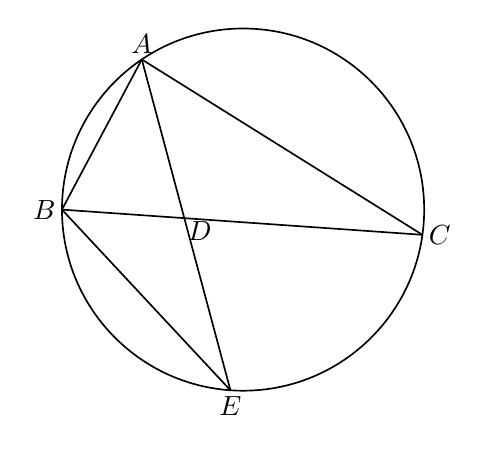
\begin{tikzpicture}[scale=1.15, semithick, line join=round]
  \coordinate (O) at (0,0);
  \coordinate (B) at (180:2);
  \coordinate (C) at (-8:2);
  \coordinate (A) at (124:2);
  \coordinate (E) at (266:2);
  \coordinate (D) at (intersection of A--E and B--C);

  \draw (O) circle[radius=2];

  \draw (A) -- (B);
  \draw (A) -- (C);
  \draw (B) -- (C);
  \draw (A) -- (E);
  \draw (B) -- (E);

  \node[above, inner sep=2pt] at (A) {$A$};
  \node[left, inner sep=2pt] at (B) {$B$};
  \node[right, inner sep=2pt] at (C) {$C$};
  \node[below right, inner sep=1pt] at (D) {$D$};
  \node[below, inner sep=2pt] at (E) {$E$};
\end{tikzpicture}
\end{center}
\nopagebreak[4]
\Needspace{4\baselineskip}
\textbf{解析}
\Needspace{5\baselineskip}
（1）因 $AD$ 平分 $\angle BAC$，且 $E$ 在 $AD$ 的延长线上，
\nopagebreak[4]
\[\angle BAE=\angle EAC=\angle DAC.\]
\Needspace{5\baselineskip}
又 $A$、$B$、$C$、$E$ 四点共圆，$\angle AEB$ 与 $\angle ACB$（即 $\angle ACD$）是同弧 $AB$ 所对的圆周角，故
\nopagebreak[4]
\[\angle AEB=\angle ACD.\]
\Needspace{5\baselineskip}
两个角对应相等，故
\nopagebreak[4]
\[\triangle ABE\sim\triangle ADC\]
（对应关系为 $A\leftrightarrow A$，$E\leftrightarrow C$，$B\leftrightarrow D$）。

\Needspace{5\baselineskip}
（2）由（1）的相似得
\nopagebreak[4]
\[\frac{AB}{AD}=\frac{AE}{AC}\iff AB\cdot AC=AD\cdot AE.\]
\Needspace{5\baselineskip}
又
\nopagebreak[4]
\[S_{\triangle ABC}=\frac12AB\cdot AC\sin\angle BAC.\]
\Needspace{5\baselineskip}
题设 $S_{\triangle ABC}=\dfrac12AD\cdot AE$，结合上式得
\nopagebreak[4]
\[\frac12AB\cdot AC\sin\angle BAC=\frac12AB\cdot AC,\]
\Needspace{5\baselineskip}
因 $AB\cdot AC>0$，故 $\sin\angle BAC=1$。而 $\angle BAC\in(0,\pi)$，故
\nopagebreak[4]
\[\angle BAC=\frac{\pi}{2}=90^\circ.\]

【图注】原页图形中 $BC$ 接近直径，与 $\angle BAC=90^\circ$ 相符；但证明只能依据题设条件。

\gkanswer{答案：（1）证明见解析；（2）$\angle BAC=90^\circ$。}

\end{answer}
\begin{answer}
\gksolhead{23}{}

\textbf{题目}：

已知 $P$ 为半圆 $C:\begin{cases}x=\cos\theta,\\y=\sin\theta,\end{cases}$（$\theta$ 为参数，$0\leqslant\theta\leqslant\pi$）上的点，点 $A$ 的坐标为 $(1,0)$，$O$ 为坐标原点，点 $M$ 在射线 $OP$ 上，线段 $OM$ 与 $C$ 的弧 $\overset{\frown}{AP}$ 的长度均为 $\dfrac{\pi}{3}$。

（1）以 $O$ 为极点，$x$ 轴的正半轴为极轴建立极坐标系，求点 $M$ 的极坐标；

（2）求直线 $AM$ 的参数方程。

\Needspace{4\baselineskip}
\textbf{解析}
\Needspace{5\baselineskip}
（1）半圆 $C$ 的半径为 $1$，$A(1,0)$ 对应参数 $\theta=0$。弧 $\overset{\frown}{AP}$ 的长为 $\dfrac{\pi}{3}$，由弧长公式 $l=R\theta$（此处 $R=1$）得圆心角
\nopagebreak[4]
\[\angle AOP=\frac{\pi}{3},\]
故 $P$ 对应的参数 $\theta=\dfrac\pi3$（在 $0\leqslant\theta\leqslant\pi$ 内唯一），射线 $OP$ 的极角为 $\dfrac\pi3$。
\Needspace{5\baselineskip}
又 $|OM|=\dfrac\pi3$，故 $M$ 的极坐标为
\nopagebreak[4]
\[(\rho,\theta)=\left(\frac{\pi}{3},\ \frac{\pi}{3}\right).\]

\Needspace{5\baselineskip}
（2）由（1），$M$ 的直角坐标为
\nopagebreak[4]
\[x_M=\frac\pi3\cos\frac\pi3=\frac\pi6,\qquad y_M=\frac\pi3\sin\frac\pi3=\frac{\sqrt3\pi}{6}.\]
\Needspace{5\baselineskip}
直线 $AM$ 过 $A(1,0)$、$M\left(\dfrac\pi6,\dfrac{\sqrt3\pi}{6}\right)$，取方向向量
\nopagebreak[4]
\[\overrightarrow{AM}=\left(\frac\pi6-1,\ \frac{\sqrt3\pi}{6}\right),\]
\Needspace{5\baselineskip}
故参数方程为
\nopagebreak[4]
\[\begin{cases}x=1+\left(\dfrac{\pi}{6}-1\right)t,\\[6pt] y=\dfrac{\sqrt3\pi}{6}t,\end{cases}\quad(t\ \text{\text{为参数}}).\]
核对：$t=0$ 给 $A(1,0)$，$t=1$ 给 $M\left(\dfrac\pi6,\dfrac{\sqrt3\pi}{6}\right)$，$t$ 取遍 $\mathbf R$ 时取遍整条直线。

\gkanswer{答案：（1）$M\left(\dfrac{\pi}{3},\dfrac{\pi}{3}\right)$；（2）$\begin{cases}x=1+\left(\dfrac{\pi}{6}-1\right)t,\\y=\dfrac{\sqrt3\pi}{6}t,\end{cases}$（$t$ 为参数）。}

\end{answer}
\begin{answer}
\gksolhead{24}{}

\textbf{题目}：

已知 $a$，$b$，$c$ 均为正数，证明：$a^2+b^2+c^2+\left(\dfrac1a+\dfrac1b+\dfrac1c\right)^2\geqslant6\sqrt3$，并确定 $a$，$b$，$c$ 为何值时，等号成立。

\Needspace{4\baselineskip}
\textbf{解析}
\Needspace{5\baselineskip}
由三元均值不等式
\nopagebreak[4]
\[a^2+b^2+c^2\geqslant3\sqrt[3]{a^2\cdot b^2\cdot c^2}=3(abc)^{\frac23},\]
\nopagebreak[4]
\[\frac1a+\frac1b+\frac1c\geqslant3\sqrt[3]{\frac1{abc}}=\frac{3}{(abc)^{\frac13}},\]
\Needspace{5\baselineskip}
故
\nopagebreak[4]
\[\left(\frac1a+\frac1b+\frac1c\right)^2\geqslant\frac{9}{(abc)^{\frac23}}.\]
\Needspace{5\baselineskip}
令 $t=(abc)^{\frac23}>0$（$a,b,c>0$），则
\nopagebreak[4]
\[a^2+b^2+c^2+\left(\frac1a+\frac1b+\frac1c\right)^2\geqslant3t+\frac9t.\]
\Needspace{5\baselineskip}
再由二元均值不等式
\nopagebreak[4]
\[3t+\frac9t\geqslant2\sqrt{3t\cdot\frac9t}=2\sqrt{27}=6\sqrt3,\]
\Needspace{5\baselineskip}
两式连起来即得
\nopagebreak[4]
\[a^2+b^2+c^2+\left(\frac1a+\frac1b+\frac1c\right)^2\geqslant6\sqrt3.\]

\textbf{等号条件}：第一处等号需 $a=b=c$；第二处等号需 $3t=\dfrac9t$，即 $t^2=3$，$t=\sqrt3$。由 $a=b=c$ 得 $t=(a^3)^{\frac23}=a^2$，故 $a^2=\sqrt3$，$a=3^{\frac14}=\sqrt[4]{3}$。
\Needspace{5\baselineskip}
即当且仅当
\nopagebreak[4]
\[a=b=c=\sqrt[4]{3}\]
时等号成立。核对：此时 $a^2+b^2+c^2=3\sqrt3$，$\dfrac1a+\dfrac1b+\dfrac1c=3\cdot3^{-\frac14}$，平方为 $\dfrac{9}{\sqrt3}=3\sqrt3$，左边 $=6\sqrt3$，与结论一致。

\gkanswer{答案：证明见解析；当且仅当 $a=b=c=\sqrt[4]{3}$ 时等号成立。}

\end{answer}